\documentclass{standalone}
\usepackage{tikz}
\usetikzlibrary{patterns, positioning}


\begin{document}
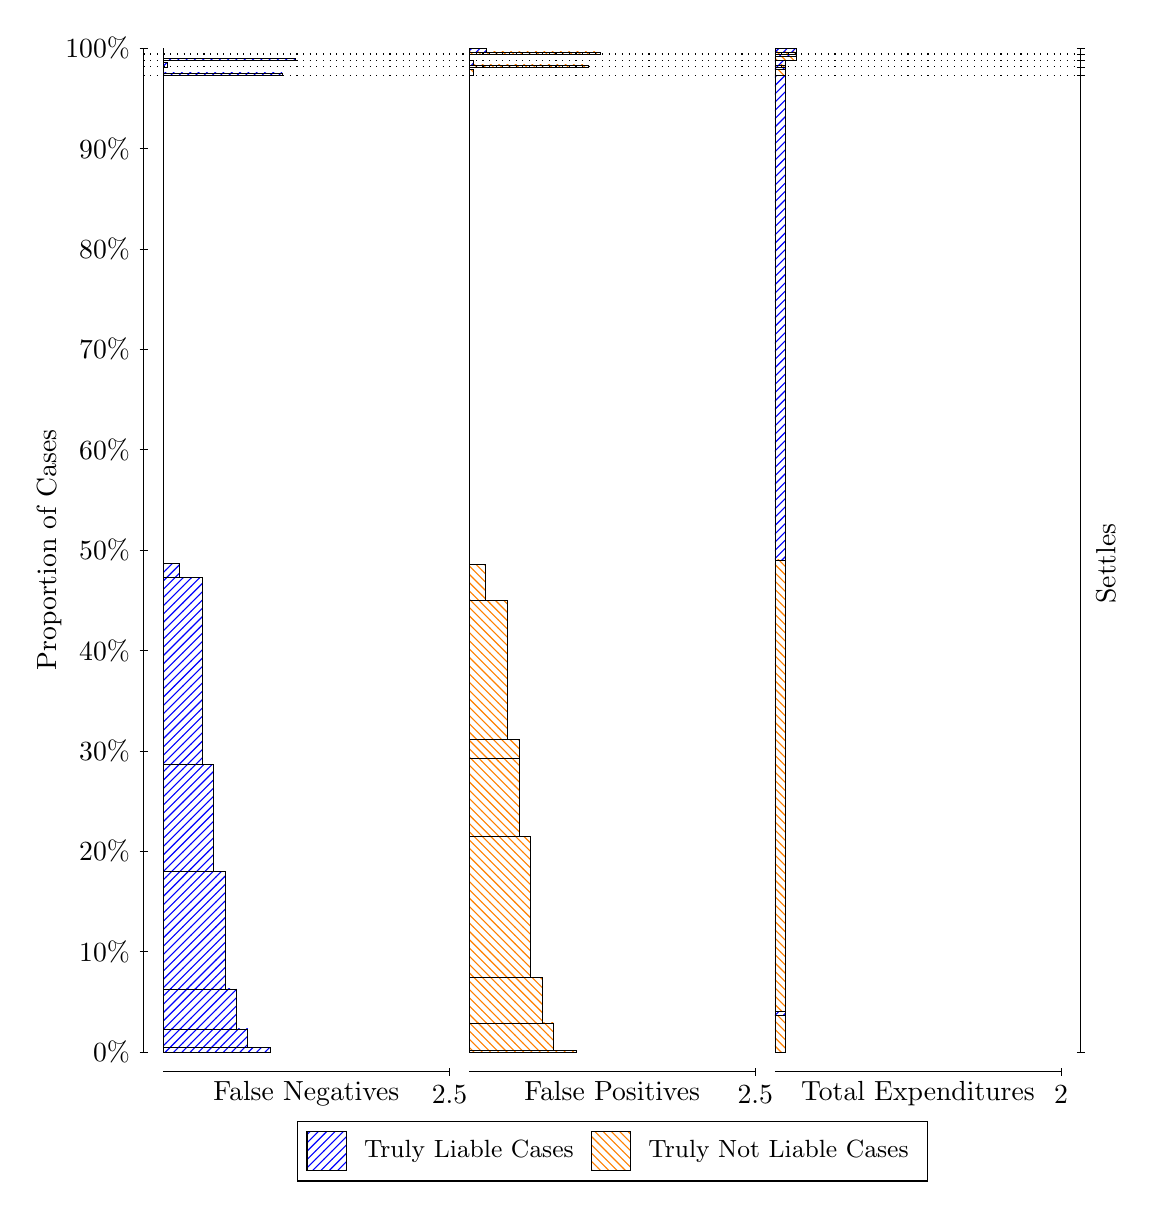
\begin{tikzpicture}
\draw[black, very thin] (1.5,1.75) -- (1.5,14.5);
\node[rotate=90, text=black, anchor=center] at (0.3, 8.125) {Proportion of Cases};
\draw[black, very thin] (1.45,1.75) -- (1.55,1.75);
\node[text=black, anchor=east] at (1.45, 1.75) {0\%};
\draw[black, very thin] (1.45,3.025) -- (1.55,3.025);
\node[text=black, anchor=east] at (1.45, 3.025) {10\%};
\draw[black, very thin] (1.45,4.3) -- (1.55,4.3);
\node[text=black, anchor=east] at (1.45, 4.3) {20\%};
\draw[black, very thin] (1.45,5.575) -- (1.55,5.575);
\node[text=black, anchor=east] at (1.45, 5.575) {30\%};
\draw[black, very thin] (1.45,6.85) -- (1.55,6.85);
\node[text=black, anchor=east] at (1.45, 6.85) {40\%};
\draw[black, very thin] (1.45,8.125) -- (1.55,8.125);
\node[text=black, anchor=east] at (1.45, 8.125) {50\%};
\draw[black, very thin] (1.45,9.4) -- (1.55,9.4);
\node[text=black, anchor=east] at (1.45, 9.4) {60\%};
\draw[black, very thin] (1.45,10.675) -- (1.55,10.675);
\node[text=black, anchor=east] at (1.45, 10.675) {70\%};
\draw[black, very thin] (1.45,11.95) -- (1.55,11.95);
\node[text=black, anchor=east] at (1.45, 11.95) {80\%};
\draw[black, very thin] (1.45,13.225) -- (1.55,13.225);
\node[text=black, anchor=east] at (1.45, 13.225) {90\%};
\draw[black, very thin] (1.45,14.5) -- (1.55,14.5);
\node[text=black, anchor=east] at (1.45, 14.5) {100\%};

\draw[black, very thin] (13.4,1.75) -- (13.4,14.5);
\draw[black, very thin] (13.35,1.75) -- (13.45,1.75);
\node[anchor=west] at (13.35, 1.75) {};
\draw[black, very thin] (13.35,14.155) -- (13.45,14.155);
\node[anchor=west] at (13.35, 14.155) {};
\draw[black, very thin] (13.35,14.261) -- (13.45,14.261);
\node[anchor=west] at (13.35, 14.261) {};
\draw[black, very thin] (13.35,14.346) -- (13.45,14.346);
\node[anchor=west] at (13.35, 14.346) {};
\draw[black, very thin] (13.35,14.424) -- (13.45,14.424);
\node[anchor=west] at (13.35, 14.424) {};
\draw[black, very thin] (13.35,14.5) -- (13.45,14.5);
\node[anchor=west] at (13.35, 14.5) {};

\draw[black, very thin, pattern color=blue, pattern=north east lines] (1.75,1.75) rectangle (3.1125,1.8051);
\draw[black, very thin, pattern color=blue, pattern=north east lines] (1.75,1.8051) rectangle (2.8218,2.0425);
\draw[black, very thin, pattern color=blue, pattern=north east lines] (1.75,2.0425) rectangle (2.6765,2.55);
\draw[black, very thin, pattern color=blue, pattern=north east lines] (1.75,2.55) rectangle (2.5312,4.0404);
\draw[black, very thin, pattern color=blue, pattern=north east lines] (1.75,4.0404) rectangle (2.3858,5.3992);
\draw[black, very thin, pattern color=blue, pattern=north east lines] (1.75,5.3992) rectangle (2.2405,7.7809);
\draw[black, very thin, pattern color=blue, pattern=north east lines] (1.75,7.7809) rectangle (1.9498,7.9596);
\draw[black, very thin, pattern color=orange, pattern=north west lines] (1.75,7.9596) rectangle (1.75,14.155);
\draw[black, very thin, pattern color=blue, pattern=north east lines] (1.75,14.155) rectangle (3.2578,14.183);
\draw[black, very thin, pattern color=orange, pattern=north west lines] (1.75,14.183) rectangle (1.75,14.261);
\draw[black, very thin, pattern color=blue, pattern=north east lines] (1.75,14.261) rectangle (1.8045,14.322);
\draw[black, very thin, pattern color=orange, pattern=north west lines] (1.75,14.322) rectangle (1.75,14.346);
\draw[black, very thin, pattern color=blue, pattern=north east lines] (1.75,14.346) rectangle (3.4213,14.373);
\draw[black, very thin, pattern color=orange, pattern=north west lines] (1.75,14.373) rectangle (1.75,14.424);
\draw[black, very thin, pattern color=orange, pattern=north west lines] (1.75,14.424) rectangle (1.75,14.45);
\draw[black, very thin, pattern color=blue, pattern=north east lines] (1.75,14.45) rectangle (1.75,14.5);
\draw[black, very thin, pattern color=orange, pattern=north west lines] (5.6333,1.75) rectangle (6.9958,1.7667);
\draw[black, very thin, pattern color=orange, pattern=north west lines] (5.6333,1.7667) rectangle (6.7052,2.1206);
\draw[black, very thin, pattern color=orange, pattern=north west lines] (5.6333,2.1206) rectangle (6.5598,2.696);
\draw[black, very thin, pattern color=orange, pattern=north west lines] (5.6333,2.696) rectangle (6.4145,4.492);
\draw[black, very thin, pattern color=orange, pattern=north west lines] (5.6333,4.492) rectangle (6.2692,5.4759);
\draw[black, very thin, pattern color=orange, pattern=north west lines] (5.6333,5.4759) rectangle (6.2692,5.7223);
\draw[black, very thin, pattern color=orange, pattern=north west lines] (5.6333,5.7223) rectangle (6.1238,7.4814);
\draw[black, very thin, pattern color=orange, pattern=north west lines] (5.6333,7.4814) rectangle (5.8332,7.9453);
\draw[black, very thin, pattern color=blue, pattern=north east lines] (5.6333,7.9453) rectangle (5.6333,14.155);
\draw[black, very thin, pattern color=orange, pattern=north west lines] (5.6333,14.155) rectangle (5.6878,14.233);
\draw[black, very thin, pattern color=blue, pattern=north east lines] (5.6333,14.233) rectangle (5.6333,14.261);
\draw[black, very thin, pattern color=orange, pattern=north west lines] (5.6333,14.261) rectangle (7.1412,14.286);
\draw[black, very thin, pattern color=blue, pattern=north east lines] (5.6333,14.286) rectangle (5.6878,14.346);
\draw[black, very thin, pattern color=orange, pattern=north west lines] (5.6333,14.346) rectangle (5.6333,14.397);
\draw[black, very thin, pattern color=blue, pattern=north east lines] (5.6333,14.397) rectangle (5.6333,14.424);
\draw[black, very thin, pattern color=orange, pattern=north west lines] (5.6333,14.424) rectangle (7.3047,14.45);
\draw[black, very thin, pattern color=blue, pattern=north east lines] (5.6333,14.45) rectangle (5.8513,14.5);
\draw[black, very thin, pattern color=orange, pattern=north west lines] (9.5167,1.75) rectangle (9.6529,2.2139);
\draw[black, very thin, pattern color=blue, pattern=north east lines] (9.5167,2.2139) rectangle (9.6529,2.269);
\draw[black, very thin, pattern color=orange, pattern=north west lines] (9.5167,2.269) rectangle (9.6529,8.0004);
\draw[black, very thin, pattern color=blue, pattern=north east lines] (9.5167,8.0004) rectangle (9.6529,14.155);
\draw[black, very thin, pattern color=orange, pattern=north west lines] (9.5167,14.155) rectangle (9.6529,14.233);
\draw[black, very thin, pattern color=blue, pattern=north east lines] (9.5167,14.233) rectangle (9.6529,14.261);
\draw[black, very thin, pattern color=orange, pattern=north west lines] (9.5167,14.261) rectangle (9.6529,14.286);
\draw[black, very thin, pattern color=blue, pattern=north east lines] (9.5167,14.286) rectangle (9.6529,14.346);
\draw[black, very thin, pattern color=orange, pattern=north west lines] (9.5167,14.346) rectangle (9.7892,14.397);
\draw[black, very thin, pattern color=blue, pattern=north east lines] (9.5167,14.397) rectangle (9.7892,14.424);
\draw[black, very thin, pattern color=orange, pattern=north west lines] (9.5167,14.424) rectangle (9.7892,14.45);
\draw[black, very thin, pattern color=blue, pattern=north east lines] (9.5167,14.45) rectangle (9.7892,14.5);
\draw[black, dotted] (1.5,14.155) -- (13.4,14.155);
\draw[black, dotted] (1.5,14.261) -- (13.4,14.261);
\draw[black, dotted] (1.5,14.346) -- (13.4,14.346);
\draw[black, dotted] (1.5,14.424) -- (13.4,14.424);
\draw[black, very thin] (1.75,1.5) -- (5.3833,1.5);
\node[text=black, anchor=north] at (3.5667, 1.5) {False Negatives};
\draw[black, very thin] (5.3833,1.45) -- (5.3833,1.55);
\node[text=black, anchor=north] at (5.3833, 1.45) {2.5};

\draw[black, very thin] (5.6333,1.5) -- (9.2667,1.5);
\node[text=black, anchor=north] at (7.45, 1.5) {False Positives};
\draw[black, very thin] (9.2667,1.45) -- (9.2667,1.55);
\node[text=black, anchor=north] at (9.2667, 1.45) {2.5};

\draw[black, very thin] (9.5167,1.5) -- (13.15,1.5);
\node[text=black, anchor=north] at (11.333, 1.5) {Total Expenditures};
\draw[black, very thin] (13.15,1.45) -- (13.15,1.55);
\node[text=black, anchor=north] at (13.15, 1.45) {2};

\node[text=black, centered, rotate=90] at (13.72, 7.9525) {Settles};





\draw (7.449999999999999,1.5) node[draw=none] (baseCoordinate) {};
\begin{scope}[align=center]
        \matrix[scale=0.5, draw=black, below=0.5cm of baseCoordinate, nodes={draw}, column sep=0.1cm]{
            \node[rectangle, draw, minimum width=0.5cm, minimum height=0.5cm, pattern color=blue, pattern=north east lines] {}; &
            \node[draw=none, font=\small, text=black] (B) {Truly Liable Cases}; &
            \node[rectangle, draw, minimum width=0.5cm, minimum height=0.5cm, pattern color=orange, pattern=north west lines] {}; &
            \node[draw=none, font=\small, text=black] (B) {Truly Not Liable Cases}; \\
            };
\end{scope}

\end{tikzpicture}
\end{document}